
\ifx \globalmark \undefined %% This is default.
	\documentclass[twoside,openright,11pt,a4paper]{report}

%\compiler avec xelatex
%\usepackage[applemac]{inputenc}
\usepackage[T1]{fontenc}
\usepackage[utf8]{inputenc} %latin1 est possible
%\usepackage[latin1]{inputenc} %latin1 est possible
\usepackage[UKenglish]{babel}
\usepackage{lettrine}

%\usepackage[text={13cm,20cm},centering]{geometry}
\usepackage [squaren, Gray, mediumqspace]{SIunits}
\usepackage [top=2cm, bottom=2cm, left=2cm, right=2cm ]{geometry}

\renewcommand{\familydefault}{cmss}
\addto\captionsenglish{ \renewcommand\chaptername{Solutions of Chapte}}

\usepackage{graphicx}
\usepackage{amsmath}
\usepackage{amsfonts}
\usepackage{amssymb}
\usepackage{amsthm}
\usepackage{bm}
\usepackage{color}

\newcommand{\real}{\mathbb{R}}
\newcommand{\mb}{\mathbf}
\newcommand{\bos}{\boldsymbol}

\def \RR {I \! \! R}

\newcommand{\e}{\begin{equation}}  
\newcommand{\ee}{\end{equation}}
\newcommand{\eqn}{\begin{eqnarray}} 
\newcommand{\eeqn}{\end{eqnarray}} 
\newcommand{\eqnn}{\begin{eqnarray*}} 
\newcommand{\eeqnn}{\end{eqnarray*}} 

\newcommand{\bpm}{\begin{pmatrix}}
\newcommand{\epm}{\end{pmatrix}}

%\newcommand{\{\c c}}{\c c}

\newcommand{\bma}{\left(\begin{array}}
\newcommand{\ema}{\end{array}\right)} 
\newcommand{\hh}{\hspace{2mm}}
\newcommand{\hd}{\hspace{5mm}}
\newcommand{\hu}{\hspace{1cm}}
\newcommand{\vv}{\vspace{2mm}}
\newcommand{\vd}{\vspace{5mm}}
\newcommand{\vm}{\vspace{-2mm}}
\newcommand{\teq}{\triangleq}
%\newcommand{\qedb}{\,$\Box$}
\newcommand{\blanc}{$\left. \right.$}
\newcommand{\frts}[2]%
         {\frac{{\textstyle #1}}{{\textstyle #2}}}

\newcommand{\bindex}[3]%
{
\renewcommand{\arraystretch}{0.5}
\begin{array}[t]{c}
#1\\
{\scriptstyle #2}\\
{\scriptstyle #3}
\end{array}
\renewcommand{\arraystretch}{1}
}

\theoremstyle{definition}
\newtheorem{exemple}{{\bf Exemple}}[chapter]
\newtheorem{theoreme}[exemple]{{\bf Th{é}or{è}me}}
\newtheorem{propriete}[exemple]{{\bf Propri{é}t{é}}}
\newtheorem{definition}[exemple]{{\bf D{é}finition}}
\newtheorem{remarque}[exemple]{{\bf Remarque}}
\newtheorem{remarques}[exemple]{{\bf Remarques}}
\newtheorem{lemme}[exemple]{{\bf Lemme}}
\newtheorem{hypothese}[exemple]{{\bf Hypoth{è}se}}
\newtheorem{exercice}{{\bf Exercice}}[chapter]

\newcommand{\xqedhere}[2]{%
 \rlap{\hbox to#1{\hfil\llap{\ensuremath{#2}}}}}

\newcommand{\xqed}[1]{%
 \leavevmode\unskip\penalty9999 \hbox{}\nobreak\hfill
 \quad\hbox{\ensuremath{#1}}}

\newcommand{\gf}{\fg\,\,}

\newcommand{\cata}[1] %
     {\renewcommand{\arraystretch}{0.5}
     \begin{array}[t]{c} \longrightarrow \\ {#1} \end{array}
     \renewcommand{\arraystretch}{1}}

\usepackage[isu]{caption}
%\usepackage[font=small,format=plain,labelfont=bf,up,textfont=it,up]{caption}
\setlength{\captionmargin}{60pt}

\newcommand{\cqfd}
{%
\mbox{}%
\nolinebreak%
\hfill%
\rule{2mm}{2mm}%
\medbreak%
\par%
}

\pagestyle{headings}

\renewcommand{\sectionmark}[1]{%
\markright{\thesection.\ #1}{}}

\renewcommand{\chaptermark}[1]{%
\markboth{\chaptername\ \thechapter.\ #1}{}}

\makeatletter 
\def\@seccntformat#1{\csname the#1\endcsname.\;} 
\makeatother

\title{ {\Huge {\textbf{Modélisation et analyse  \\ \vspace{4mm} des systèmes dynamiques }}} \\ \vspace{4cm} G. Bastin}

%\title{ {\Huge {\textbf{Modelisation et analyse  \\ \vspace{4mm} des systemes dynamiques }}} \\ \vspace{4cm} G. Bastin}


\date{\today}
	\begin{document} %% Crashes if put after (one of the many mysteries of LaTeX?).
\else 
	\documentclass{standalone}
	\begin{document}
\fi

\graphicspath{ {Chapitre10/images/} }

\setcounter{chapter}{9}
\chapter{Commandabilité et planification de trajectoires}
\chaptermark{Commandabilité et planification de trajectoires}\label{complantraj}



\lettrine[lines=1]{\bf D}{}ans les trois chapitres précédents, nous avons étudié en
détail  le comportement des systèmes dynamiques {\it libres} 
dont les entrées sont {\it constantes}~: $\dot x = f(x,\bar u)$.
Dans ce dernier chapitre, nous allons considérer des systèmes
dynamiques {\it commandés} $\dot x = f(x,u)$ et nous
intéresser en particulier à l'existence et la détermination de
fonctions d'entrées $u(t)$ pouvant varier au cours du temps et
permettant de piloter le système dans l'espace d'état et d'en
planifier les trajectoires.

\section{Définitions}

Dans la pratique, il arrive souvent que l'on désire conduire un
système dynamique d'un état initial $x_0$ à un état final
$x_f$.  C'est ce qu'on appelle un {\it problème de planification de trajectoire}. Pour résoudre un tel problème, il faut qu'il existe au
moins une fonction d'entrée $u(t)$ produisant une trajectoire
du système passant par les états $x_0$ et $x_f$.
\begin{definition}{{\bf Etats atteignables}}

Pour le système dynamique $\dot x = f(x,u)$ , l'état final $x_f$ est atteignable à partir de l'état initial $x_0$ s'il existe un
temps fini $T$ et une fonction d'entrée $u(t) : [t_0,t_0 +T]
\rightarrow \mathbb{R}^n$ tels que $x(t_0+T,x_0,u) = x_f$. 
\qed
\end{definition} 
Cette notion d'atteignabilité conduit au concept de commandabilité
d'un système dynamique explicité dans
la définition suivante.\\\\\\

\begin{definition}{{\bf Commandabilité}}

Le système $\dot x = f(x,u)$ est {\it localement commandable} en $x_f$ s'il
existe un voisinage de $x_f$ tel que $x_f$ soit atteignable à
partir de chaque élément du voisinage.

Le système est {\it globalement 
commandable} si tout état $x_f \in \mathbb{R}^n$ est atteignable à
partir de tout état initial $x_0 \in \mathbb{R}^n$.
\qed
\end{definition}
L'objet de ce chapitre est d'étudier la commandabilité et la planification de trajectoires des systèmes dynamiques $\dot x = f(x,u)$. Comme nous le verrons, l'analyse de
l'atteignabilité et de la commandabilité est totalement élucidée
pour les systèmes linéaires alors qu'il reste de nombreuses
questions ouvertes pour les systèmes non linéaires. D'autre
part le problème de la planification des trajectoires est
entièrement résolu pour les systèmes linéaires, alors qu'on n'en
connait la solution que pour une classe restreinte de systèmes
non linéaires que l'on appelle {\it systèmes (différentiellement)
plats} et qui sont, en un certain sens, équivalents à des
systèmes linéaires.


\section{Commandabilité : systèmes linéaires}

Pour vérifier si un système linéaire $\dot x = Ax + Bu$ est
complètement commandable, on peut utiliser l'un des deux critères
donnés par le théorème suivant.
\begin{theoreme} {\bf Commandabilité des systèmes linéaires}
\label{linear}


Le système linéaire $\dot x = Ax + Bu$ est complètement commandable
si et seulement si l'un des deux critères équivalents suivants est
satisfait~:
\begin{enumerate}
\item (Critère de Kalman) La matrice ${\cal C} = (B \hh AB \hh A^2B
\dots A^{(n-1)}B)$ est ré-gulière (cette matrice est appelée {\it
matrice de commandabilité}); 
\item (Critère de Popov-Belevitch-Hautus) Le rang de la matrice $(sI-A \hh B)$
est égal à $n$ pour tout $s \in {\mathbb {C}}$. \qed
\end{enumerate}
\end{theoreme}
Si un système linéaire n'est pas complètement commandable, on peut
définir une transformation d'état pour mettre la partie non
commandable du vecteur d'état en évidence.

Supposons que la matrice de commandabilité soit de rang $d < n$.  On
définit une matrice $T = (T_a \hh T_b)$ telle que $T_a$ contienne $d$
colonnes linéairement indépendantes de $\cal C$ et $T_b$ complète la
matrice par $n-d$ vecteurs indépendants des colonnes de $T_a$. La
matrice inverse $T^{-1}$ peut dès lors s'écrire~:
\eqnn
T^{-1} = \bma{c} U_a \\ U_b \ema
\eeqnn
où les sous matrices $U_a$ et $U_b$ sont choisies telles que~:
\eqnn
T^{-1}T = \bma{cc} U_aT_a & U_aT_b \\ U_bT_a & U_bT_b \ema = 
\bma{cc} I_d & 0 \\ 0 & I_{n-d} \ema
\eeqnn
On définit la transformation d'état~:
\eqnn
z = \bma{c} z_a \\ z_b \ema = \bma{c} U_ax \\ U_bx \ema
\eeqnn
Dans ces nouvelles variables d'état, on a le modèle d'état suivant~:
\eqnn
\dot z_a &=& U_aAT_az_a + U_aAT_bz_b + U_aBu \\
\dot z_b &=& U_bAT_bz_b
\eeqnn
En effet $U_bT_a=0$ implique que $U_bB = 0$ et $U_bAT_a=0$ car les colonnes de $B$ et de $AT_a$ sont des combinaisons linéaires des colonnes de $T_a$.
On observe que la partie $z_b$ du vecteur d'état n'est pas influencée
par l'entrée $u$~: elle représente la partie non commandable de l'état
du système.

\section{Commandabilité : systèmes non-linéaires}

L'étude de la commandabilité des systèmes non-linéaires est beaucoup
plus compliquée que celle des systèmes linéaires. Nous commençons
cette étude par l'examen des conclusions que l'on peut tirer de la
commandabilité du linéarisé d'un système non-linéaire au voisinage d'un
équilibre. 
\begin{theoreme} {\bf Commandabilité locale (1)}\label{linear}


Considérons le linéarisé du système $\dot x = f(x,u)$ autour d'un
équilibre $(\bar x, \bar u)$~:
\eqn \label{lin}
\dot x = Ax +Bu \hd
\text{avec} \hd
A = ({\frac{\partial f}{\partial x}})_{(\bar x, \bar u)} \;\; \text{et} \;\; B = 
({\frac{\partial f}{\partial u}})_{(\bar x, \bar u)}.
\eeqn
Si le système linéaire (\ref{lin}) est commandable, alors, pour tout
$\epsilon > 0$, l'ensemble des états $x_f$ atteignables à partir de $\bar
x$ avec des entrées $u(t)$ : $u(t) - \bar u < \epsilon$, contient un
voisinage de $\bar x$.
\qed

\end{theoreme}
Cette propriété locale de commandabilité des systèmes non-linéaires a
une portée limitée. Comme nous allons le voir dans l'exemple suivant, il
existe en effet des systèmes non-linéaires complètement
commandables, dont le linéarisé n'est pas commandable au voisinage
de l'équilibre !\\

\begin{exemple}{\bf Une voiture automobile} \label{voiture}

Considérons une voiture automobile de type \og traction avant \fg~dont les roues avant sont à la fois motrices et directrices. Le modèle cinématique s'écrit~:
\eqnn
\dot \xi_1 &=& \sin \theta_1 \cos \theta_2 u_1 \\
\dot \xi_2 &=& -\cos \theta_1 \cos \theta_2 u_1 \\
\dot \theta_1 &=& \sin \theta_2 u_1 \\
\dot \theta_2 &=& u_2
\eeqnn
où $(\xi_1,\xi_2)$ désignent les coordonnées cartésiennes du milieu de
l'essieu arrière, $\theta_1$ l'orientation du chassis, $\theta_2$
l'orientation des roues avant, $u_1$ la vitesse de propulsion et
$u_2$ la vitesse d'orientation des roues avant.

Ce système possède une infinité d'équilibres non isolés de la forme
$(\bar \xi_1, \bar \xi_2, \bar \theta_1,$ $\bar \theta_2, 0, 0)$. Les
matrices $(A,B)$ du linéarisé du système autour d'un quelconque de ces
équlibres s'écrivent~:
\eqnn
A = 0 \hu B = \bma{cc} \sin {\bar \theta_1} \cos {\bar \theta_2} & 0 \\
-\cos {\bar \theta_1} \cos {\bar \theta_2} & 0 \\
\sin {\bar \theta_2} & 0 \\ 0 & 1 \ema
\eeqnn
On observe immédiatement que le système linéarisé n'est pas
commandable (rang ${\cal C} = 2$) alors que l'intuition physique indique à
l'évidence qu'une voiture automobile est un système dynamique
commandable qui, dans un environnement sans obstacle, peut être
manoeuvré pour aller de n'importe quelle position initiale à n'importe
quelle position finale.
\qed

\end{exemple}

Comme l'indique cet exemple, un système non-linéaire peut posséder
des propriétés de commandabilité qui ne sont pas apparentes dans le
linéarisé. L'analyse de ces propriétés est facilitée par l'usage de
concepts et de notations de géométrie différentielle qui sont
brièvement résumés en annexe. Nous en commençons l'étude par la
présentation d'une procédure qui permet, lorsqu'un système n'est {\textit {pas}} commandable, de mettre les variables d'état non-commandables
en évidence.

Supposons que, pour un système $\dot x = f(x,u)$ donné, il existe une
transformation d'état $z = \phi(x)$ telle que, dans les nouvelles
variables d'état, le système s'écrive comme suit~:
\eqnn
z = \bma{c} z_a \\ z_b \ema \hu 
\left \{
\begin{tabular}{ll}
$\dot z_a = \tilde f_a(z_a, z_b, u)$ \\
$\dot z_b = \tilde f_b(z_b)$ 
\end{tabular}
\right.
\eeqnn
Il est clair, dans ce cas, que la partie $z_b$ du vecteur d'état n'est pas
influencée par l'entrée $u$ et que le système n'est donc pas
commandable. En voici un exemple simple.

\begin{exemple}{\bf Un réacteur chimique}

Considérons un réacteur chimique isotherme et parfaitement mélangé
dans lequel se déroule la réaction réversible~:
\eqnn
2X_1 \longleftrightarrow X_2 + X_3 
\eeqnn
Le réacteur est alimenté par l'espèce $X_1$ avec un débit volumétrique
constant et une concentration variable. Le modèle d'état s'écrit~:
\eqnn
\dot x_1 &=& -2k_1x_1^2 + 2k_2x_2x_3 - dx_1 + du \\
\dot x_2 &=& k_1x_1^2 - k_2x_2x_3 - dx_2 \\
\dot x_3 &=& k_1x_1^2 - k_2x_2x_3 - dx_3
\eeqnn
Soit la transformation d'état linéaire~:
\eqnn
\begin{tabular}{lcl}
$z_1 = x_1$ &  & $x_1 = z_1$ \\
$z_2 = x_2$ & $\longleftrightarrow$  & $x_2 = z_2$ \\
$z_3 = x_2 - x_3 $ &  & $x_3 = z_2 - z_3$ 
\end{tabular}
\eeqnn
Dans les nouvelles variables d'état, le modèle se réécrit~;
\eqnn
\dot z_1 &=& -2k_1z_1^2 + 2k_2z_2(z_2 - z_3) - dz_1 + du \\
\dot z_2 &=& k_1z_1^2 - k_2z_2(z_2 - z_3) - dz_2 \\
\dot z_3 &=& -dz_3
\eeqnn
Le système n'est donc pas commandable car les trajectoires de $z_3$
(qui est la différence entre les concentrations des espèces $X_2$ et
$X_3$) ne peuvent être influencées par l'entrée $u$ (qui est la
concentration d'alimentation de l'espèce $X_1$).
\qed

\end{exemple}
Une condition suffisante d'existence d'une partie non-commandable de
l'état est donnée dans le théorème suivant pour les systèmes affines
en l'entrée~:
\eqn
\dot x = f(x) + \sum_{j=1}^m g_j(x)u_j \label{affine}
\eeqn
\begin{theoreme}


Si, dans un voisinage $U$ d'un point $x_0$, il existe une distribution
$\Delta(x)$ régulière de dimension $d$ telle que~:
\begin{enumerate}
\item $\Delta(x)$ est involutive
\item $\Delta(x)$ contient $\mbox{ span} \{ g_1(x), g_2(x), \dots
,g_m(x)\}$
\item $\Delta (x)$ est invariante par rapport à $f(x)$ et $g_1(x), g_2(x), \dots
,g_m(x)$,
\end{enumerate}
alors il existe une transformation d'état $\phi : U \longrightarrow
V=\phi(U)$ telle que, dans les nouvelles variables d'état $z=\phi(x)$, le
système (\ref{affine}) se réécrit~:
\eqnn
\dot z_a &=& \tilde f_a(z_a, z_b) +  \sum_{j=1}^m \tilde g_j(z_a,
z_b)u_j\\ \dot z_b &=& \tilde f_b(z_b) 
\eeqnn
avec dim $z_b = (n-d)$.
\qed

\end{theoreme}
Le théorème suivant permet alors de déterminer la plus petite
distribution $\Delta^*(x)$ qui vérifie les conditions ci-dessus et
donc de déterminer la dimension maximum de la partie
non-commandable. 

\begin{theoreme} \label{procedure}


Dans un voisinage $U$ de $x_0$, on définit la séquence de
distributions~:
\eqnn
\Delta_0(x) &=& \mbox{ span} \{g_1(x), g_2(x), \dots , g_m(x) \} \\
\Delta_k(x) &=& \Delta_{k-1}(x) + [f(x),\Delta_{k-1}(x)] + 
\sum_{j=1}^m [g_j(x),\Delta_{k-1}(x)].
\eeqnn
Alors $\Delta^*(x) =
\Delta_{k^*}(x)$ avec $k^*$ le plus petit entier tel que
$\Delta_{k^*}(x)$ est régulière sur $U$ et invariante par rapport à $f(x)$
et $g_1(x), g_2(x), \dots ,g_m(x)$. Si toutes les distributions
$\Delta_k(x), 0 \leq k \leq k^*$ sont régulières sur U, alors $k^* \leq n$.
\qed 
\end{theoreme}
La dimension de $\Delta^*$ porte le nom de {\it rang d'atteignabilité}
du système au voisinage de $x_0$.  L'énoncé du  théorème
\ref{procedure} contient implicitement une procédure pour la
détermination du rang d'atteignabilité qui consiste à générer
successivement les distributions $\Delta_k(x)$. La procédure s'arrête
dès qu'on en trouve une qui est régulière et invariante par rapport à $f$
et aux $g_i$. Il n'est pas nécessaire de vérifier que
cette distribution est involutive. Il est intéressant aussi de constater
que, dans le cas d'un système linéaire $\dot x = Ax + Bu$, on a~:
\eqnn
\Delta_k = \mbox{ span }\{B \hh AB \dots A^{k-1}B \}
\eeqnn
et donc que le rang d'atteignabilité coïncide avec le rang de la matrice
de commandabilité ${\cal C}$.

Un système dont le rang d'atteignabilité est maximum (c'est-à-dire égal
à $n$) au voisinage de $x_0$ possède alors une propriété de
commandabilité locale semblable à celle du théorème \ref{linear}, même
si $x_0$ n'est pas un état d'équilibre et même si le linéarisé du système
n'est pas commandable. 

\begin{theoreme} {\bf Commandabilité locale (2)}


Pour le système (\ref{affine}), il existe un voisinage de $x_0$ dont tous
les états sont atteignables à partir de $x_0$ si et seulement si le rang
d'atteignabilité du système au voisinage de $x_0$ est égal à $n$.
\qed

\end{theoreme}
Enfin on a la propriété de commandabilité complète pour une
sous-classe de systèmes.
\begin{theoreme} {\bf Commandabilité
complète}


Si $f(x) \in \mbox{ span} \{g_1(x), g_2(x), \dots , g_m(x) \}$
pour tout $x \in \mathbb{R}^n$ (ceci est vrai en particulier si $f(x) = 0$) et si le
rang d'atteignabilité vaut $n$ au voisinage de tout $x \in \mathbb{R}^n$, alors le
système (\ref{affine}) est complètement commandable.
\qed 
\end{theoreme}
Ces deux théorèmes sont illustrés dans l'exemple suivant.
\begin{exemple}{\bf Une voiture automobile}


Considérons à nouveau le modèle de la voiture automobile de l'exemple
\ref{voiture} qui s'écrit~:
\eqnn
\dot x = g_1(x)u_1 + g_2(x)u_2
\eeqnn
avec~:
\eqnn
g_1(x) = \bma{c} \sin \theta_1 \cos \theta_2 \\ 
-\cos \theta_1 \cos \theta_2 \\ \sin \theta_2 \\ 0 \ema \hu g_2(x) =
\bma{c} 0 \\ 0 \\ 0 \\ 1 \ema
\eeqnn
On calcule les crochets de Lie~:
\eqnn
g_3(x) = [g_1(x),g_2(x)] &=& \bma{c} -\sin \theta_1 \sin \theta_2 \\ 
\cos \theta_1 \sin \theta_2 \\ \cos \theta_2 \\ 0 \ema \\
g_4(x) = [g_3(x),g_1(x)] &=& \bma{c} \cos \theta_1 \\ \sin \theta_1 \\ 0
\\0 \ema
\eeqnn
On vérifie que $f(x) = 0$ et que la matrice $[g_1(x), g_2(x), g_3(x),
g_4(x)]$ est régulière pour tout $x$ dans $\mathbb{R}^4$. Ces deux conditions
suffisent pour que les hypothèses des deux théorèmes précédents
soient vérifiées. La voiture automobile est donc bien complètement
commandable même si son modèle linéarisé ne l'est pas.  
\qed 

\end{exemple} 
Les résultats présentés dans cette section peuvent
paraître restrictifs car ils ne s'appliquent qu'à des systèmes affines en
l'entrée. Leur portée est cependant plus générale car un
système quelconque $\dot x = f(x,u)$ peut toujours être augmenté par
une {\it extension dynamique} pour le rendre affine en l'entrée. Il suffit
en effet de considérer $u$ comme un ensemble additionnel de variables
d'état et de définir un nouveau vecteur $v$ de variables d'entrée telles
que~: 
\eqnn \dot x &=& f(x,u) \\
\dot u &=& v
\eeqnn
Avec le vecteur d'état augmenté $\xi^T = (x^T,u^T)$, le système
s'écrit~:
\eqn
&&\dot \xi = \varphi(\xi) + \sum_{j=1}^m g_jv_j = \varphi(\xi) +
Gv \label{augm}\\
&\mbox{où : }&\varphi(\xi) = \bma{c} f(x,u) \\ 0 \ema \hu G = \bma{c} 0
\\ I_m \ema \nonumber
\eeqn
La commandabilité du système augmenté (\ref{augm}), que l'on peut vérifier avec les théorèmes précédents, est évidemment suffisante pour garantir la commandabilité du système original.

\section{Planification de trajectoires}

Dans les sections précédentes, nous avons étudié les conditions et les
critères qui permettent de savoir si un système est commandable. Il
est évidemment encore plus intéressant de pouvoir déterminer la
fonction d'entrée $u(t)$ qui permet effectivement de conduire le
système d'un état initial $x_0$ à un état final $x_f$ en un temps
raisonnable. C'est le problème de la {\it planification de trajectoire}
que nous allons traiter maintenant.

\subsection{Systèmes mono-entrée sous forme de Brunovski}
Nous considérons ici les systèmes affines en l'entrée $\dot x = f(x) +
g(x)u, u \in \mathbb{R}$ qui peuvent se mettre sous forme de Brunovski et qui
sont caractérisés par le théorème suivant.
\begin{theoreme}


Un système $\dot x = f(x) +
g(x)u$ peut être mis sous forme de Brunovski dans un domaine $U
\subset R^n$ si et seulement si~:
\begin{itemize}
\item[1)] La matrice ${\cal D} = [g(x) \hh ad_fg(x) \hh ad_f^2g(x) \dots
ad_f^{n-1}g(x)]$ est régulière $\forall x \in U$;
\item[2)] La distribution $\Delta(x) = \mbox{ span }\{g(x) 
 \dots ad_f^{n-2}g(x)\}$ est involutive sur $U$. \qed
\end{itemize}
\end{theoreme}
Si ces conditions sont satisfaites, il existe une transformation d'état
$z=\varphi(x)$, $z : U \longrightarrow V$ telle que le système se
réécrive sous la forme triangulaire (dite de Brunovski)~:
\begin{align} \label{bruno}
\dot z_1 &= z_2 \nonumber \\
\dot z_2 &= z_3  \\
&\vdots \nonumber \\
\dot z_n &= \alpha(z) + \beta(z)u \hu \beta(z) \neq 0 \hh \forall z \in
V \nonumber
\end{align}
On déduit immédiatement de ce théorème qu'un {\it système linéaire} mono-entrée
$\dot x = Ax + bu$ peut être mis sous forme de Brunovski si et
seulement si il est complètement commandable. En effet, dans ce cas,
la matrice ${\cal D}$ est la matrice de commandabilité du système~:
\eqnn
{\cal D} = {\cal C} = [b \hh Ab \hh A^2b \dots A^{(n-1)}b]
\eeqnn
et la distribution $\Delta$ est nécessairement involutive puisqu'elle ne
contient que des vecteurs constants. Il existe alors une transformation
{\it linéaire} d'état~:
\eqnn
z = Tx
\eeqnn
telle que le système se réécrit sous forme de Brunovski~:
\eqnn
\dot z_i &=& z_{i+1} \hu i = 1, \dots , n \\
\dot z_n &=& - \sum_{i=1}^n \alpha_i z_i + \beta u
\eeqnn
La matrice $T$ est définie comme suit~:
\eqnn
T=\bma{c} h^T \\ h^TA \\ \vdots \\ h^TA^{n-1} \ema
\eeqnn
où le vecteur $h$ est la dernière colonne de la transposée de l'inverse de la matrice de
commandabilité ${\cal C}^{-T}$.

Une fois que le système, qu'il soit linéaire ou non-linéaire, est sous
forme de Brunovski, le problème de planification de trajectoire devient
très facile à résoudre. Nous commençons par en montrer la
solution pour le cas particulier d'un système quelconque de dimension
deux.

\begin{exemple} {\bf Un système de dimension 2}


Soit le système~:
\eqnn
\dot x_1 &=& f_1(x_1,x_2) + g_1(x_1,x_2)u \\
\dot x_2 &=& f_2(x_1,x_2) + g_2(x_1,x_2)u
\eeqnn
Le problème est de trouver une fonction d'entrée $u(t)$ qui conduise
ce système d'un état initial $(x_1(0), x_2(0))$ à un état final
$(x_1(T), x_2(T))$.

On suppose qu'il
existe une transformation d'état~: 
\eqnn z_1 &=& \phi_1(x_1,x_2) \\
z_2 &=& \phi_2(x_1,x_2)
\eeqnn
qui met le système sous forme de Brunovski~:
\eqn
\dot z_1 &=& z_2 \label{bruno1}\\
\dot z_2 &=& \alpha(z_1,z_2) + \beta(z_1,z_2)u \label{bruno2}
\eeqn
Le problème est maintenant de trouver une fonction $u(t)$ qui conduise
le système (\ref{bruno1})-(\ref{bruno2}) de l'état initial $z_1(0) =
\phi_1(x_1(0),x_2(0))$, $z_2(0) =
\phi_2(x_1(0),x_2(0))$ à l'état final $z_1(T) =
\phi_1(x_1(T),x_2(T))$,  $z_2(T) =
\phi_2(x_1(T),x_2(T))$. Pour la variable d'état $z_1(t)$,
on définit une trajectoire polynomiale de la forme~:
\eqnn
z_1(t) = \lambda_3(\frac{t}{T})^3 + \lambda_2(\frac{t}{T})^2 +
\lambda_1(\frac{t}{T}) + \lambda_0
\eeqnn
où les coefficients $\lambda_i$ sont pour le moment inconnus. On
déduit de la forme de Brunovski que la trajectoire de $z_2(t)$ doit être
de la forme~:
\eqnn
z_2(t) = \dot z_1(t) = \frac{3}{T}\lambda_3(\frac{t}{T})^2 + 
\frac{2}{T}\lambda_2(\frac{t}{T}) + \frac{1}{T}\lambda_1
\eeqnn
En explicitant les expressions de $z_1(t)$ et $z_2(t)$ aux instants $t=0$
et $t=T$, on observe alors que les coefficients $\lambda_i$ sont
solution du système d'équations linéaires~:
\eqn
\bma{cccc} 1 & 0 & 0 & 0 \\ 0 & \frac{1}{T} & 0 & 0 \\ 1 & 1 & 1 & 1 \\ 0 &
\frac{1}{T} & \frac{2}{T} & \frac{3}{T} \ema \bma{c} \lambda_0 \\ 
\lambda_1 \\ \lambda_2 \\ \lambda_3 \ema 
= \bma{c} z_1(0) \\ z_2(0) \\ z_1(T) \\ z_2(T) \ema \label{sl}
\eeqn
Les $\lambda_i$ étant ainsi déterminés, on connait maintenant une
trajectoire $z_1(t), z_2(t)$ qui relie les états initial et final désirés et on
peut calculer l'entrée $u(t)$ correspondante~: 
\eqnn
u(t) = \frac{\dot z_2(t) - \alpha(z_1(t),z_2(t))}{\beta(z_1(t),z_2(t))}
\eeqnn
avec
\eqnn
\dot z_2(t) = \frac{6}{T^2}\lambda_3(\frac{t}{T}) +
\frac{2}{T^2}\lambda_2
\eeqnn
Le problème de la planification de trajectoire est ainsi résolu.
\qed

\end{exemple}
Le cas particulier d'un système de dimension $2$ que nous venons d'étudier se généralise facilement en dimension $n$. Rappelons qu'on suppose que le système est sous forme de Brunovski~:
\eqnn
\dot z_1 &=& z_2 \\
\dot z_2 &=& z_3 \\
&\vdots& \\
\dot z_n &=& \alpha(z) + \beta(z)u \hu \beta(z) \neq 0 
\eeqnn
Il suffit de définir, pour $z_1(t)$, une trajectoire polynomiale de la forme~:
\eqnn
z_1(t) = \sum_{i=0}^{2n-1} \lambda_i(\frac{t}{T})^{i}
\eeqnn
En calculant les dérivées successives de $z_1(t)$, on obtient les expressions de $z_j(t)$, $j=2,\dots,n$~:
\eqnn
z_j(t) = \sum_{i=j-1}^{2n-1}\frac{i!}{(i-j+1)!}\frac{\lambda_i}{T^{j-1}}(\frac{t}{T})^{-j+1}
\eeqnn
En explicitant ensuite ces expressions aux instants $t=0$ et $t=T$, on obtient un système d'équations linéaires qui généralise le système (\ref{sl}) et permet de calculer les $\lambda_i$. Il ne reste plus alors qu'à calculer l'entrée $u(t)$~:
\eqnn
u(t) = \frac{\dot z_n(t) - \alpha(z(t))}{\beta(z(t))}
\eeqnn

\begin{remarque}


Nous avons présenté ci-dessus une solution du problème de planification basée sur l'utilisation de fonctions polynomiales d'ordre $2n-1$ pour générer les trajectoires du système. Le choix de telles fonctions polynomiales n'a cependant rien d'impératif. D'une manière plus générale, comme on peut le déduire aisément des développements précédents, on peut utiliser des combinaisons linéaires de $2n-1$ fonctions linéairement indépendantes quelconques.

\end{remarque}

\subsection{Systèmes linéaires multi-entrées}
Nous considérons maintenant des systèmes linéaires multi-entrées de la forme suivante~:
\eqnn
\dot x = Ax + Bu \hspace{6mm} x \in \mathbb{R}^n \hspace{6mm} u \in \mathbb{R}^m
\eeqnn
On suppose que rang($B$) $= m$ et que le système est commandable. On définit
les {\it indices de commandabilité} $\delta_1, \delta_2, \dots ,
\delta_m$~:
\eqnn
\delta_i = \mbox{ card}[m_j \geq i \,\, : \,\, j \geq 0]
\eeqnn
avec
\eqnn
m_0 &=& \mbox{ rang}B\\
m_1 &=& \mbox{ rang}[B,AB] - \mbox{ rang}B\\
\vdots\\
m_{n-1} &=& \mbox{ rang}[B,\dots,A^{n-1}B]-\mbox{ rang}[B, \dots,
A^{n-2}B]
\eeqnn
Par définition, on a~:
\eqnn
\delta_1 \geq \delta_2 \geq \dots \geq \delta_m \hspace{4mm} \mbox{et}
\hspace{4mm} \sum_{j=1}^m \delta_j = n
\eeqnn
Il existe alors une transformation d'état $z=Tx$ qui permet de mettre le
système sous une forme de Brunovski généralisée constituée de $m$ blocs ayant chacun la forme triangulaire suivante~:
\eqn
\dot z_{j1} &=& z_{j2} \nonumber \\
\dot z_{j2} &=& z_{j3} \nonumber \\
&\vdots& \hspace{2cm} \label{brunomulti}\\
\dot z_{j\delta_{j-1}} &=& z_{j\delta_j} \nonumber\\
\dot z_{j\delta_j} &=&  \bindex {\sum}{j=1,m}{i=1,\delta_j} \alpha_{ji} z_{ji} + \sum_{k=1,m} \beta_{jk} u_k \nonumber
\eeqn
Le vecteur d'état $z$ est formé des $n$ variables $z_{ji}$, $j=1 \dots m$, $i=1 \dots\delta_j$.
La matrice $G=[\beta_{jk}]$ est carrée et inversible. Cette forme de Brunovski multi-entrées peut alors être utilisée, comme dans le cas mono-entrée, pour résoudre des problèmes de planification de trajectoire.

\subsection{Sorties de Brunovski}
 En introduisant la notation $y_j = z_{j1}$, le modèle d'état \eqref{brunomulti} peut aussi être écrit sous la forme plus compacte  
\eqnn
\dot y_{j}^{(\delta_{j}+1)} = \bindex {\sum}{j=1,m}{i=1,\delta_j} \alpha_{ji} y_j^{(i)} + \sum_{k=1,m} \beta_{jk} u_k \hu j=1, \dots , m 
\eeqnn
c'est-à-dire sous la forme de $m$ équations différentielles linéaires d'ordre $(\delta_{j}~+1)$. Les variables $y_j$ sont des combinaisons linéaires de l'état $x$ et sont appelées {\em sorties de Brunovski}. On remarque que le nombre de sorties de Brunovski est égal au nombre d'entrées du système.

\subsection{Systèmes non-linéaires multi-entrées}
Considérons maintenant un système non-linéaire multi-entrées, affine en l'entrée~:
\eqnn
\dot x = f(x) + \sum_{j=1}^m g_j(x)u_j.
\eeqnn
Pour ce système, on peut étendre la notion de forme de Brunovski multi-entrées si il existe une transformation d'état non-linéaire $z = T(x)$ qui permette de mettre le système sous la forme bloc-triangulaire
\eqnn
\dot z_{j1} &=& z_{j2} \nonumber \\
\dot z_{j2} &=& z_{j3} \nonumber \\
&\vdots& \hspace{2cm} \hu \hu j= 1, \dots, m\\
\dot z_{j\delta_{j-1}} &=& z_{j\delta_j} \nonumber\\
\dot z_{j\delta_j} &=&   \alpha_{j} (z) + \sum_{k=1,m} \beta_{jk}(z) u_k \nonumber
\eeqnn
où le vecteur d'état $z$ est formé de $n$ variables $z_{ji}$, $j=1 \dots m$, $i=1 \dots\delta_j$ et la matrice carrée $G(z) = [\beta_{jk}(z)]$ est inversible. Dans ce cas, les sorties de Brunovski sont des fonctions non-linéaires de l'état ($y_j = z_{1j} = h_j(x)$) et le modèle peut s'écrire sous la forme d'un système d'équations différentielles nonlinéaires
\eqn
\dot y_{j}^{(\delta_{j}+1)} = \alpha_{j} (z) + \sum_{k=1,m} \beta_{jk}(z) u_k \hu j=1, \dots , m \label{brunomultinonlin}
\eeqn
où le vecteur $z$ est maintenant défini comme suit :
\eqnn
z = (y_1, \dot y_1, \dots, y_1^{(\delta_1)},  \dots, y_m, \dot y_m, \dots , y_m^{(\delta_m)}).
\eeqnn
Contrairement au cas linéaire, les systèmes non-linéaires commandables ne peu-vent pas toujours être mis sous une telle forme de Brunovski multi-entrées. Il sort du cadre de ce texte de discuter des conditions sous lesquelles la transformation est possible. C'est d'ailleurs une question qui n'est pas complètement clarifiée et qui fait encore l'objet de recherches actives à l'heure actuelle. Nous nous limiterons à présenter les deux exemples ci-dessous. Le premier est un exemple simple où le système est naturellement sous la forme de Brunovski multi-entrées (\ref{brunomultinonlin}). Le deuxième exemple est plus complexe. Il montrera un système commandable pour lequel il faut, par une {\em extension dynamique},  utiliser une forme de Brunovski augmentée dont la dimension est supérieure à la dimension du système lui-même.

\begin{exemple} {\bf Un robot manipulateur}


Considérons à nouveau le modèle du robot manipulateur à deux degrés de liberté que nous avons étudié au chapitre 2 (Exemple 2.2). En examinant le modèle, on observe facilement qu'il est d'emblée donné sous une forme de Brunovski multi-entrées avec les deux coordonnées de position $y_1 = x_1$ et $y_2 = \theta_2$ comme sorties de Brunovski. Pour éviter d'inverser explicitement la matrice d'inertie, on peut écrire le modèle comme suit sous forme matricielle :
\eqnn
\left(\begin{array}{c}\ddot y_1 \\\ddot y_2\end{array}\right) = \left(\begin{array}{cc}m_1 + m_2 & m_2b\cos y_2 \\m_2b \cos y_2 & I_2 + m_2b^2\end{array}\right)^{-1}  \left(\begin{array}{c}m_2b \dot y_2^2 \sin y_2 + u_1 \\-m_2bg_o \sin y_2 +u_2 \end{array}\right).
\eeqnn
Les indices de commandabilité sont ici $\delta_1$ = $\delta_2$ = 2. La matrice $G(z)$ est l'inverse de la matrice d'inertie. \qed

\end{exemple}

\begin{exemple}{\bf Dynamique d'une fusée}


Au chapitre 2 (Exemple 2.1), nous avons établi le modèle de la dynamique d'une fusée comme suit :
\begin{itemize}
\item Equations de translation
\eqnn
m\ddot{x} &=& (F_1 + F_2)\cos\theta \\ 
m\ddot{y} &=& (F_1 + F_2)\sin\theta - mg_0 
\eeqnn
\item Equation de rotation
\eqnn
I\ddot{\theta} = (F_2 - F_1)d\sin\alpha 
\eeqnn
\end{itemize}
\noindent 
Dans ces équations, $(x,y)$ est la position du centre de masse de la fusée, $\theta$ l'angle de la fusée par rapport à l'horizontale, $F_{1}$ et $F_{2}$ les poussées des réacteurs, $m$ la masse de la fusée, $I$ son moment d'inertie, $d$ et $\alpha$ des paramètres géométriques et $g_0$ l'accélération de la gravité. Pour simplifier l'écriture sans perte de généralité, nous définissons les entrées
\eqnn
u_1 = \dfrac{F_1 + F_2}{m}, \hu u_2 = \dfrac{(F_2 - F_1)d \sin\alpha}{I}.
\eeqnn
Avec ces notations, le modèle d'état s'écrit simplement~:
\begin{align*}
\ddot x &= u_1 \cos \theta \\
\ddot y &= u_1 \sin \theta - g_0 \\
\ddot \theta &= u_2
\end{align*}

\end{exemple}
Ce système est complètement commandable en vertu du Théorème 10.10. Intuitivement, on peut penser que les coordonnées $x$ et $y$ sont les sorties de Brunovski. Nous allons voir que cette intuition est justifiée, mais qu'elle implique une définition étendue de la notion de forme de Brunovski.

Calculons les dérivées troisièmes des coordonnées $x$ et $y$ :
\begin{align*}
\stackrel{\dots}{x} &= \dot u_1 \cos \theta - u_1 \dot \theta \sin \theta \\
\stackrel{\dots}{y} &= \dot u_1 \sin \theta + u_1 \dot \theta \cos \theta
\end{align*}
Il est clair que ces expressions ne peuvent pas être utilisées pour bâtir une forme de Brunovski du type \eqref{brunomultinonlin} car elles ne contiennent pas l'entrée $u_2$. Par contre si on considère l'entrée $u_1$ comme une variable d'état supplémentaire et qu'on ajoute deux intégrateurs à l'entrée du système, alors on peut montrer que le système étendu possède une forme de Brunovski multi-entrées avec les coordonnées $y_1 = x$ et $y_2 = y$ comme sorties de Brunovski. Le système étendu s'écrit donc comme suit :
\begin{align} \label{etendufusee}
&\ddot x = u_1 \cos \theta \nonumber \\
&\ddot y = u_1 \sin \theta \nonumber \\
&\ddot \theta = u_2 \\
&\ddot u_1 = w_1 \nonumber
\end{align}
C'est un système qui est maintenant de dimension 8 (alors que le système de départ était de dimension 6) avec deux entrées $w_1$ et $u_2$. Calculons les dérivées 4-ièmes des sorties de Brunovski $x$ et $y$ :
\begin{align}
&\left(\begin{array}{c}\stackrel{....}{x} \\ \stackrel{....}{y} \end{array}\right) = \left(\begin{array}{c}-2\dot u_1 \dot \theta \sin \theta - u_1 \dot \theta^2 \cos \theta 
 \\ 2\dot u_1 \dot \theta \cos \theta + u_1 \dot \theta^2 \sin \theta\end{array}\right) \nonumber \\
&\hspace{4cm} + \left(\begin{array}{cc}\cos \theta & -u_1 \sin \theta \\\sin \theta & u_1 \cos \theta\end{array}\right)\left(\begin{array}{c}w_1 \\u_2\end{array}\right). \label{brunofusee}
\end{align}
Il est maintenant clair que ce système peut être écrit sous une forme de Brunovski multi-entrées de la forme :
\eqnn
\left(\begin{array}{c}\stackrel{....}{y_1} \\\stackrel{....}{y_2} \end{array}\right) = \alpha(z) + G(z) \left(\begin{array}{c}w_1 \\u_2\end{array}\right).
\eeqnn
En effet, à partir du modèle d'état \eqref{etendufusee}, les différents termes qui apparaissent dans l'équation \eqref{brunofusee} peuvent être exprimés (après un peu de calcul !) en fonction des sorties de Brunovski $y_1 = x$ et $y_2 = y$ et de leurs dérivées, comme suit :
\eqnn
 u_1 \cos \theta = \ddot y_1, \hu  u_1 \sin \theta = \ddot y_2 + g_o,
 \eeqnn
 \eqnn
\sin \theta = \dfrac{ \ddot y_2 + g_o}{\sqrt{ \ddot y_1^2 + ( \ddot y_2 + g_o)^2}}, \hu \cos \theta = \dfrac{ \ddot y_1}{\sqrt{ \ddot y_1^2 + ( \ddot y_2 + g_o)^2}}, 
\eeqnn
\eqnn
\dot \theta = \dfrac {\ddot y_1 \stackrel{...}{y_2} - (\ddot y_2 + g_o) \stackrel{...}{y_1} } {\ddot y_1^2 + ( \ddot y_2 + g_o)^2 }, 
\eeqnn
\eqnn
\dot u_1 \cos \theta = \stackrel{...}{y_1} + \dot \theta (\ddot y_2 + g_o), \hu \dot u_1 \sin \theta = \stackrel{...}{y_2} - \dot \theta \ddot y_1.
\eeqnn
D'autre part, la matrice
\eqnn
G(z) = \left(\begin{array}{cc}\cos \theta & -u_1 \sin \theta \\\sin \theta & u_1 \cos \theta\end{array}\right)
\eeqnn
est régulière pour tout $\theta$ et pour tout $u_1 \neq 0$ (c-à-d tant que la poussée totale $F_1 + F_2$ des moteurs de la fusée n'est pas nulle). \qed \\

Les systèmes non-linéaires qui peuvent être mis sous une forme de Brunovski multi-entrées, moyennant éventuellement une extension dynamique,  sont appelés dans la littérature, {\em systèmes (différentiellement) plats} parce qu'ils sont, en un certain sens, équivalents à des systèmes linéaires comme le montre la méthode de calcul de la planification des trajectoires. Pour cette raison, les sorties de Brunovski sont parfois aussi appelées {\em sorties plates}.

\section{Annexe : formules de géométrie différentielle}

\begin{enumerate}
\item Champ de vecteur
\eqnn
f(x) = \bma{c} f_1(x)\\ f_2(x) \\ \vdots \\ f_n(x) \ema
\eeqnn
\vspace{5mm}
\item Crochet de Lie
\eqnn
[ f(x) , g(x) ] &=& \dfrac{\partial g(x)}{\partial x} f(x) - \dfrac{\partial f(x)}{\partial x} g(x) \\ && \\  \left[ f(x) , g(x) \right] &=& - [ g(x) , f(x) ]
\eeqnn
\vspace{5mm}
\item Notation itérative
\eqnn
ad_fg &=& [f,g] \\ && \\
ad_f^2g &=& [f,ad_fg] = [f, [f,g]] \\
&\vdots& \\
ad_f^kg &=& [f, ad_f^{k-1}g]
\eeqnn
\vspace{5mm}
\item Distribution = ensemble d'espaces vectoriels
\eqnn
\Delta(x) = \span \left\{ f_1(x), f_2(x), \hdots , f_d(x) \right\}
\eeqnn
\vspace{5mm}
\item Distribution $\Delta$ {\em involutive} si
$[f_1,f_2] \in \Delta \;\; \forall \;\; f_1 \in \Delta \; , \; f_2 \in \Delta$
\vspace{5mm}
\item Distribution $\Delta$ {\em invariante} par rapport à $g$ si
\eqnn
\forall \;\; f \in \Delta \;\; \Rightarrow \;\; [g,f] \in \Delta
\eeqnn
\end{enumerate}

\section{Exercices}

\begin{exercice}{\bf \em Une montgolfière\footnote{Problème extrait de "Analyse et commande de systèmes dynamiques" par F. Bonnans et P. Rouchon, Manuel de l' Ecole Polytechnique (France), édition de 2003.}}


On considère le modèle suivant pour une montgolfière : 
\eqnn
\dot\theta &=& -\frac{1}{\tau_1}\theta + u\\
\dot v &=&  -\frac{1}{\tau_2}v+\sigma\theta \\
\dot h &=& v
\eeqnn
où $\theta$ est l'écart de température de l'air par rapport à la
température d'équilibre,\\
$u$ est la commande (proportionnelle à la quantité d'énergie
utilisée pour chauffer l'air du ballon),\\
$v$ est la vitesse verticale (vitesse ascensionnelle),\\
$h$ est la hauteur.

\begin{enumerate}
\item Commenter les équations. 
\item Le système est-il commandable ?
\item Planifier une trajectoire de $\bma{c}0\\0\\h_0\ema $ à
$\bma{c}0\\0\\h_1\ema $ \ en $T=1$.
\end{enumerate}

\end{exercice}

\vspace*{3cm}
\begin{exercice}{\bf \em Un réacteur biochimique}


Soit un réacteur à volume constant (unitaire) alimenté en réactif
$A$ (débit $d$, concentration $x^{in}_A$) dans lequel se déroule
la réaction
$$
A+B \rightarrow 2B+C$$ La cinétique de la réaction est donnée par
la loi d'action des masses.
\begin{enumerate}
\item Donner une représentation d'état du système réactionnel.
\item Trouver, si c'est possible, un difféomorphisme mettant en
évidence les modes non commandables du système.  Examiner les 2
cas suivants : \subitem La commande est $d$ \subitem La commande
est $x^{in}_A$
\end{enumerate}

\end{exercice}


\vspace*{2mm}
\begin{exercice}{\bf \em Contrôle d'attitude d'un satellite}

Le contrôle de l'orientation d'un satellite (appelé contrôle d'attitude) peut avoir divers objectifs : pointer une antenne, un appareil de mesure ou un panneau solaire dans la bonne direction, éviter la déterioration par les rayons solaires d'éléments sensibles, orienter le satellite en vue de manoeuvres orbitales etc...

On considère un satellite dans l'espace dont les équations du
mouvement s'écrivent : 
\eqnn \dot x_1 &=& a_1x_2x_3+b_1u_1\\
\dot x_2 &=& a_2x_1x_3+b_2 u_2\\
\dot x_3 &=& a_3x_1x_2
\eeqnn
Etudier la commandabilité locale (Théorème 10.9) de ce système ($a_i \neq 0 \; b_i \neq 0$).
\end{exercice}

\newpage
\begin{exercice}{\bf \em Un plongeur\footnote{Problème extrait de "Analyse et commande de systèmes dynamiques" par F. Bonnans et P. Rouchon, Manuel de l' Ecole Polytechnique (France), édition de 2003.}}


On considère le modèle ci-dessous décrivant la dynamique verticale
d'un plongeur équipé d'un gilet stabilisateur contenant une
quantité réglable d'air, notée $q$ (exprimée en moles):
\eqnn
M\frac{d^2h}{dt^2} &=& Mg- \rho g\left(V_0+\frac{qRT}{P_0+ \rho h}\right)\\
\frac{dq}{dt} &=&u 
\eeqnn
avec les notations suivantes : \\

$h$ \;\;\;  : \;\; profondeur du plongeur mesurée
positivement depuis la surface
\eqnn \hspace{-3.4 cm} \left.
\begin{tabular}{lll}
$M$&:& masse du plongeur\\
$P_0$ &:& pression atmosphérique \\
$T$ &:& température\\
$R$ &:&  constante de Boltzmann\\
$\rho$ &:& masse spécifique de l'eau\\
$V_0$&:& volume du plongeur
\end{tabular}
\right\} \mbox{constantes}\\
\eeqnn
 La première équation est un bilan de force selon l'axe vertical.
 Ce bilan comprend la poussée d'Archimède $pg(V_0+V_g)$ où $V_g$
 est le volume du gilet obtenu en fonction de la pression
 $p=P_0+ \rho h$ par la loi des gaz parfaits $PV=qRT$.

 La deuxième équation représente le remplissage du gilet par l'air
 des bouteilles $(u>0)$ ou la purge du gilet $(u>0)$.
 \begin{enumerate}
 \item Montrer que le système peut être mis sous forme de
 Brunovski.
 \item Montrer que le système est commandable.
 \item On désire remonter de façon contrôlée entre deux paliers
 stabilisés.  Le palier de départ $(t=0)$ est à la profondeur
 $\bar h_1$.  Le palier d'arrivée $(t=t_f)$ est à la profondeur
 $\bar h_2$.  Indiquer comment calculer l'entrée $u(t)$ qui assure
 la transition entre ces ceux équilibres.
 \end{enumerate}

\end{exercice}

\vspace*{2mm}
\begin{exercice}{\bf \em Un robot sauteur}


On considère un \og robot sauteur \fg \; schématisé comme ci-dessous.
Ce robot est formé d'un corps de masse $M$ muni d'une jambe de
masse $m$.  
\begin{figure}[h]
\begin{center}
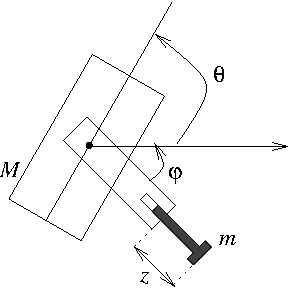
\includegraphics{robsauteur}
\end{center}
\end{figure}

\noindent La jambe est articulée et on peut en contr\^oler
l'orientation $\varphi$ et l'extension
$z$.
La conservation du moment angulaire autour du centre de masse instantané
s'écrit ($d$= constante) :
\eqnn
M\dot \theta + m (z + d)^2(\dot\theta + \dot \varphi)=0
\eeqnn
Les deux entrées de commande du système sont les vitesses d'orientation et
d'élongation de la jambe.
$$
u_1 = \dot \varphi \;\;\; (2) \hspace*{1cm} u_2 = \dot z \;\;\; (3)
$$
\begin{enumerate}
\item Ecrire les 3 équations (1) à (3) sous la forme d'un modèle d'état
dont les entrées sont $u_1$ et $u_2$.
\item Examiner si le système décrit par ce modèle est complètement
commandable.
\end{enumerate}

\end{exercice}

 
\end{document}
